\documentclass{article}
\usepackage{tikz}
\usetikzlibrary{shadows,shapes} % LATEX and plain TEX when using TikZ
\begin{document}
\tikz [even odd rule]
\draw [general shadow={fill=red}] (0,0) circle (.5) (0.5,0) circle (.5);

\tikz [even odd rule]
\filldraw [drop shadow,fill=white] (0,0) circle (.5) (0.5,0) circle (.5);

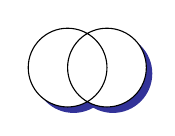
\begin{tikzpicture}[every shadow/.style={opacity=.8,fill=blue!50!black}]
\filldraw [drop shadow,fill=white] (0,0) circle (.5) (0.5,0) circle (.5);
\end{tikzpicture}

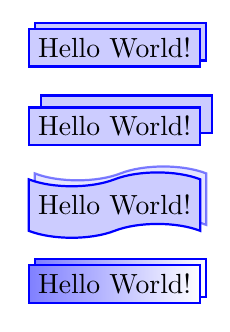
\begin{tikzpicture}
\node [copy shadow,fill=blue!20,draw=blue,thick] {Hello World!};
\node at (0,-1) [copy shadow={shadow xshift=1ex,shadow yshift=1ex},
fill=blue!20,draw=blue,thick]
{Hello World!};
\node at (0,-2) [copy shadow={opacity=.5},tape,
fill=blue!20,draw=blue,thick]
{Hello World!};
% We have to repeat the left color since shadings are not
% automatically applied to shadows
\node at (0,-3) [copy shadow={left color=blue!50},
left color=blue!50,draw=blue,thick]
{Hello World!};
\end{tikzpicture}

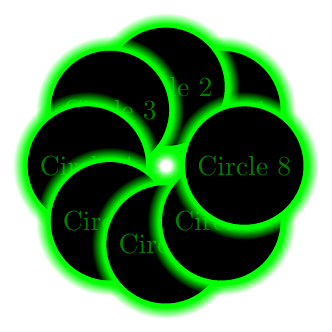
\begin{tikzpicture}
\foreach \i in {1,...,8}
\node[circle,circular glow={fill=green},fill=black,text=green!50!black]
at (\i*45:1) {Circle \i};
\end{tikzpicture}

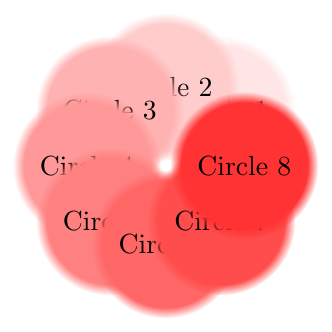
\begin{tikzpicture}
\foreach \i in {1,...,8}
\node[circle,circular glow={fill=red!\i0}]
at (\i*45:1) {Circle \i};
\end{tikzpicture}
\end{document}
